\documentclass[border=4pt]{standalone}
\usepackage{tikz}
\usetikzlibrary{positioning, arrows.meta, shapes.geometric, calc, fit, backgrounds}
\usepackage{amsmath,amssymb}
\begin{document}
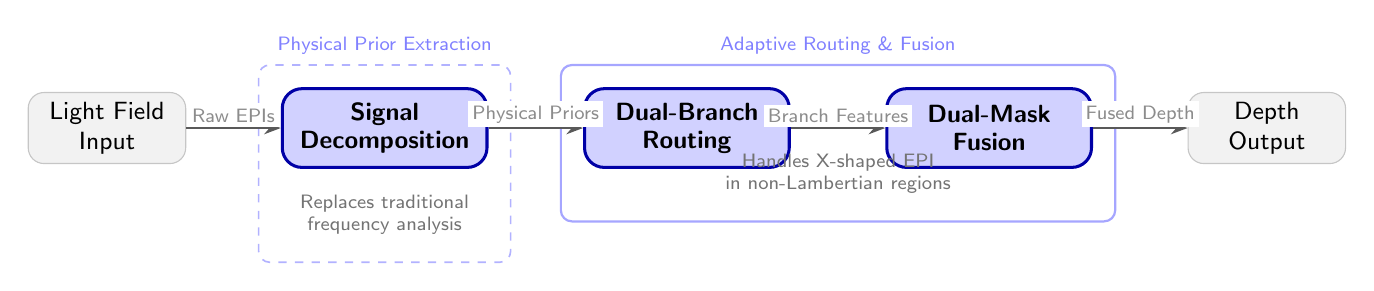
\begin{tikzpicture}[
  node distance=1.2cm and 1.2cm,
  input/.style={draw, rounded corners=2mm, minimum width=2.0cm, minimum height=0.8cm,
                fill=gray!10, draw=gray!45, align=center, font=\sffamily\small},
  innov/.style={draw, rounded corners=2.5mm, minimum width=2.6cm, minimum height=1.0cm,
                fill=blue!18, draw=blue!65!black, line width=1.1pt, align=center,
                font=\sffamily\small\bfseries},
  arr/.style={-{Stealth[length=6pt]}, thick, color=black!65},
  lbl/.style={font=\sffamily\scriptsize, text=black!45, fill=white, inner sep=1.5pt},
  gbox/.style={draw=#1, dashed, rounded corners=4pt, inner sep=8pt, line width=0.6pt},
  gbox/.default=blue!30,
  gbox_solid/.style={draw=#1, solid, rounded corners=4pt, inner sep=8pt, line width=0.8pt},
  gbox_solid/.default=blue!35,
  note/.style={font=\sffamily\scriptsize, text=black!55, align=center, inner sep=2pt}
]

% Nodes
\node[input] (m1) {Light Field\\Input};
\node[innov, right=1.2cm of m1] (m2) {\textbf{Signal}\\[-1pt]\textbf{Decomposition}};
\node[innov, right=1.2cm of m2] (m3) {\textbf{Dual-Branch}\\[-1pt]\textbf{Routing}};
\node[innov, right=1.2cm of m3] (m4) {\textbf{Dual-Mask}\\[-1pt]\textbf{Fusion}};
\node[input, right=1.2cm of m4] (m5) {Depth\\Output};

% Arrows
\draw[arr] (m1) -- node[lbl, above] {Raw EPIs} (m2);
\draw[arr] (m2) -- node[lbl, above] {Physical Priors} (m3);
\draw[arr] (m3) -- node[lbl, above] {Branch Features} (m4);
\draw[arr] (m4) -- node[lbl, above] {Fused Depth} (m5);

% Key Annotations
\node[note, below=0.25cm of m2] (note1) {Replaces traditional\\frequency analysis};
\coordinate (mid34) at ($(m3)!0.5!(m4)$);
\node[note, below=0.25cm of mid34] (note2) {Handles X-shaped EPI\\in non-Lambertian regions};

% Groups
\begin{scope}[on background layer]
  \node[gbox, fit=(m2)(note1), label={[font=\sffamily\scriptsize, text=blue!50]above:Physical Prior Extraction}] {};
  \node[gbox_solid, fit=(m3)(m4)(note2), label={[font=\sffamily\scriptsize, text=blue!50]above:Adaptive Routing \& Fusion}] {};
\end{scope}

\end{tikzpicture}
\end{document}